\documentclass{article}
\pagenumbering{arabic}
\newcommand{\newCommandName}{text to insert}
% Pages and colors used for the cover page
\usepackage{tikz-page}
\usepackage{url}
\usepackage{lastpage}

% Used for the math and code
\usepackage{amsmath}
\usepackage{listings}
\usepackage{pythonhighlight} % Got this from github! https://github.com/olivierverdier/python-latex-highlighting/blob/master/pythonhighlight.sty

% Used for the pictures
\usepackage{float}
\usepackage{graphicx}
\usepackage{mwe,tikz}\usepackage[percent]{overpic}

% For the table
\usepackage[utf8]{inputenc}
\usepackage{multirow}
\usepackage{colortbl}

\usepackage[
  top=2cm,
  bottom=2cm,
  left=3cm,
  right=2cm,
  headheight=17pt, % as per the warning by fancyhdr
  includehead,includefoot,
  heightrounded, % to avoid spurious underfull messages
]{geometry} 

% Page numbers/header
\usepackage{fancyhdr}
\definecolor{brickred}{rgb}{0.8, 0.25, 0.33}
\definecolor{cobalt}{rgb}{0.0, 0.28, 0.67}
\definecolor{cadetgrey}{rgb}{0.57, 0.64, 0.69}

% Defining the text box being used for DEPT OF ENG
\tikzset{
        secnode/.style={
                minimum height = .16in,
                minimum width = 4.16in,
                inner xsep = 2pt,
                anchor=north east,
                draw=cadetgrey,
                fill=white,
                text=brickred,
                },
        }


         
\pagestyle{plain}
\renewcommand{\headrulewidth}{0pt}
\begin{document}


% Put name data and assignment number here
\newcommand\personaldate{February 3, 2024}
\newcommand\myname{Leo Berman}
\newcommand\myemail{leo.berman@temple.edu}
\newcommand\hwnum{3}
\newcommand\mynameabbrev{L. Berman}
\newcommand\assignmenttitle{Maximum Likelihood VS. Bayesian Estimation}
\newcommand\yourclass{ECE 8527: Machine Learning and Pattern Recognition}
\begin{titlepage}
	% Drawing the border and the text box 
	\newcommand{\tikzpagelayout}{
		\draw[line width = .04in,
			color = cobalt]
		($(current page.north west)+(1in,-1in)$)
		rectangle ($(current page.south east)+(-.625in,1in)$);

		\draw[line width = .04in,
			color = brickred]
		($(current page.north west)+(.92in,-.92in)$)
		rectangle ($(current page.south east)+(-.705in,1.08in)$);
		\node[secnode] at ($(current page.north west)+(6in,-.875in)$) {\small{\textbf{DEPARTMENT OF ELECTRICAL AND COMPUTER ENGINEERING}}};
	}

	\begin{center}
		\large{Homework Assignment No. \hwnum:}\break
		\break
		\large{\textbf{HW No. \hwnum: \assignmenttitle}}\break
		\break
		\large{submitted to \:}\break
		\break
		\large{Professor Joseph Picone}\break
		\large{ECE 8527: Introduction to Pattern Recognition and Machine Learning}\break
		\large{Temple University}\break
		\large{College of Engineering}\break
		\large{1947 North 12th Street}\break
		\large{Philadelphia, Pennsylvania 19122}\break
		\break
		\large{\personaldate}\break
		\break
		\large{prepared by: }\break
		\break
		\large{\myname}\break
		\large{Email: \myemail}
	\end{center}
\end{titlepage}

\newpage
\pagestyle{fancy}
\fancyhead{}
\fancyfoot{}
\fancyhead[R,EH]{Page \thepage\ of \pageref{LastPage}}
\fancyhead[L,EH]{\mynameabbrev: HW \# \hwnum}
\fancyfoot[L,EF]{\yourclass}
\fancyfoot[R,EF]{\personaldate}
\renewcommand{\thesection}{\Alph{section}.}

\section{\MakeUppercase{Generate 11 Independent Sets of Data}}
\flushleft{First, 11 one dimensional vectors with 10$^{6}$ points, Variance = 1, and the followings means were generated:}\break
\center{0.90, 0.92, 0.94, 0.96, 0.98, 1.00, 1.02, 1.04, 1.06, 1.08, 1.10}\break
\flushleft{These were generated using the following python snippet:}\break
\begin{python}
	# generate the points for each set
    vectors = []
    for i in range(11):
        vectors.append(numpy.random.normal(loc = .9+(i*.02),scale = 1,size = 10**6))
\end{python}
\flushleft{The Maximum Likelihood Estimation was calculated for all the independent vecotrs by calculating the mean with respect to the number of points factored in with the following snippet:}\break
\begin{python}
	# create a dictionary to hold each set's means
    mean_plot_points = {}
    
    # iterate through all sets
    for i,x in enumerate(vectors):

        # keep track of the mean of that set
        mysum = 0

        # Add the set to the dictionary
        mean_plot_points[round(.90+(.02*i),2)] = []
        for j,y in enumerate(x):
            # keep track of the mean and append each mean point
            mysum+=y
            mean_plot_points[round(.90+(.02*i),2)].append(mysum/(j+1))
\end{python}
\pagebreak
\flushleft{All the plots using MLE use the following function to create the plots: }\break
\begin{python}
	def cascading_arrow(data,ylower,yhigher):
		
		# generate x_axis
		x_axis = numpy.linspace(1,10**6,10**6)
		
		# create subplots
		fig,ax = plt.subplots()

		# plot the data
		ax.plot(x_axis,data)

		# set the x-axis to a logarithmic scale
		plt.xscale("log")

		# set bounds
		plt.ylim(ylower,yhigher)
		plt.xlim(0,10**7)

		#iterate through 1,5,10,50,100,500...5*10^5,10**6
		index = 1
		for i in range(13):

			# scientific notation to be efficient with space
			if i > 10:
				pltstr = '('+"{:.0e}".format(round(x_axis[index-1],0))+','+str(round(data[index-1],2))+')'
			else:
				pltstr = '('+str(round(x_axis[index-1],0))+','+str(round(data[index-1],2))+')'
			
			# annotate stacked cascading arrows with text centered
			ha = 'center'
			if i == 0:
				xloc = x_axis[index-1]+2
			else:
				xloc = x_axis[index-1]

			if (i%2) == 0:
				ax.annotate(pltstr,xy=(x_axis[index-1],data[index-1]),xytext=(xloc,ylower+((yhigher-ylower)/14)+(i*((yhigher-ylower)/42))),arrowprops=dict(facecolor='black', shrink=.05), horizontalalignment=ha)
				index*=5
			else:
				ax.annotate(pltstr,xy=(x_axis[index-1],data[index-1]),xytext=(xloc,yhigher-((yhigher-ylower)/14)-(i*((yhigher-ylower)/42))),arrowprops=dict(facecolor='black', shrink=.2), horizontalalignment=ha)
				index*=2
\end{python}
\pagebreak
\section{\MakeUppercase{MLE for Mean=1.00 and Means=(0.90, 0.92, \ldots, 1.00) }}
\begin{figure}[!htb]
	\centering
	\begin{minipage}{0.49\textwidth}
			\centering
			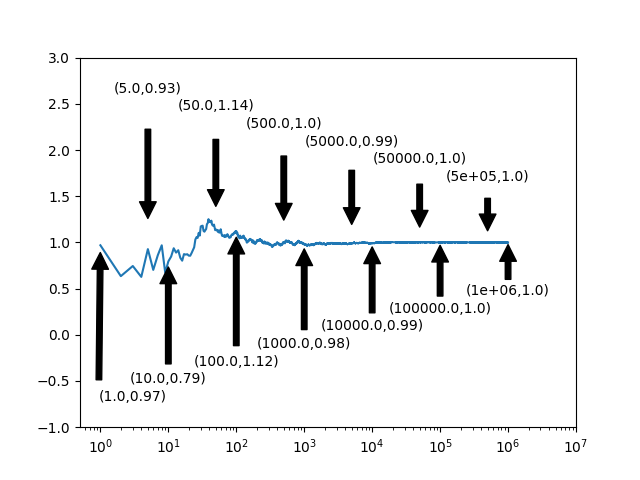
\includegraphics[width=1\linewidth]{../Q2a.png}
			\caption{(Mean = 1.00)}
	\end{minipage}\hfill
	\begin{minipage}{0.49\textwidth}
		\centering
		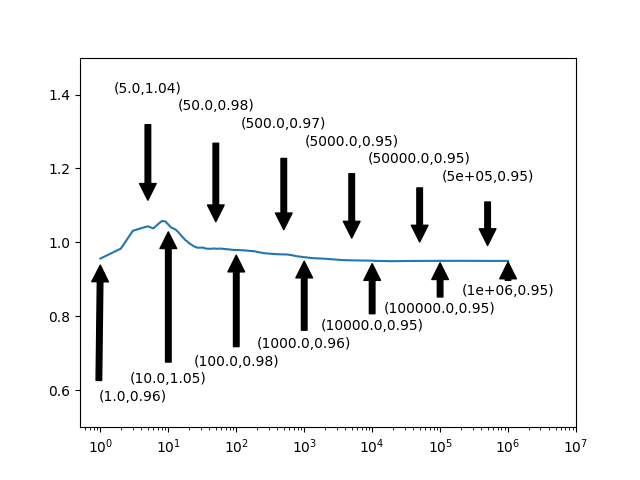
\includegraphics[width=1\linewidth]{../Q2b.png}
		\caption{(Means = 0.90, 0.92, \ldots, 0.98, 1.00)}
	\end{minipage}\hfill
\end{figure}
\flushleft{The first estimate that uses the one dimensional vector centered around one is clearly biased towards one and clearly converges to 1. However, the second estimate isn't biased towards one and clearly converges towards 0.95 which makes sense as:}\break 
\[ \dfrac{\sum_{n=0}^{5} {0.90+(.02*n)}}{6} = .95 \]
\pagebreak
\section{\MakeUppercase{MLE for Means = (0.90, 0.92, \ldots, 1.10)}}
\flushleft{Plot the maximum likelihood estimation by plotting the means of each individual vector as a function of $\dfrac{Total Points}{Total Vectors}$. In practice, this looks like taking the mean of Figure 3 and plotting it with a correlating x axis.}
\begin{figure}[!htb]
	\centering
	\begin{minipage}{0.49\textwidth}
		\centering
		\begin{tikzpicture}[      
			every node/.style={anchor=south west,inner sep=0pt},
			x=1mm, y=1mm,
		  ]   
		 \node (fig1) at (0,0)
		   {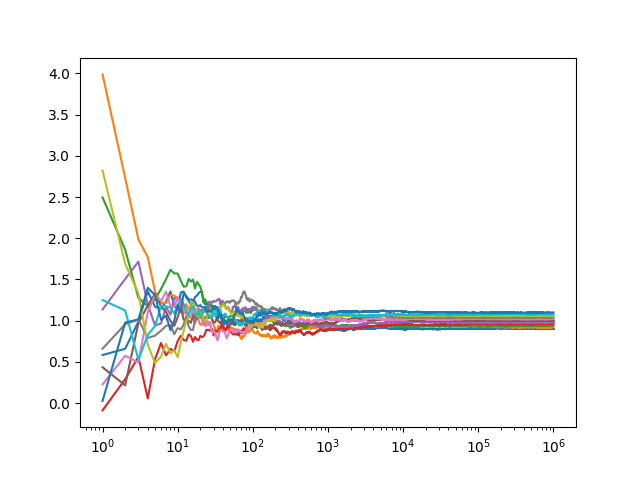
\includegraphics[scale=0.49]{../SeparateMeans.png}};
		 \node (fig2) at (33,23)
		   {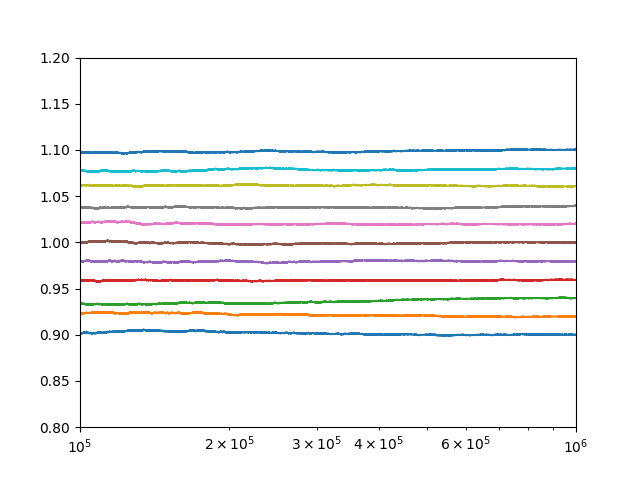
\includegraphics[scale=0.23]{../SeparateMeans_Zoomed.png}};
	\end{tikzpicture}
	\caption{Means = (0.90, 0.92, \ldots, 1.10 )}
	\end{minipage}
	\begin{minipage}{0.49\textwidth}
			\centering
			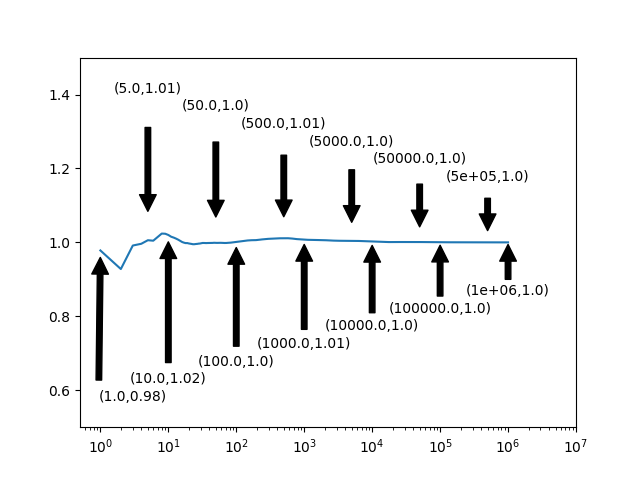
\includegraphics[width=1\linewidth]{../Q3a.png}
			\caption{Mean of Means = (0.90, 0.92, \ldots, 1.10 )}
	\end{minipage}
\end{figure}
\flushleft{When we compare the plot in Figure 4 to the plot of Figure 3, we can see that both plots converge to a mean estimation of 1.00, but not only does Figure 4 converge faster, it also has less noise. The reason that this happens is because there are more point surrounding the mean of 1.00 for Figure 4. Not only does it have access to all the points that Figure 1 has it also has access to the 10 other sets that have a combined mean of means equal to 1.00 as well.}
\pagebreak
\section{\MakeUppercase{Last sec}}

\section{\MakeUppercase{Summary}}
\end{document}